% Copyright © 2013 Martin Ueding <dev@martin-ueding.de>

% Copyright © 2012-2013 Martin Ueding <dev@martin-ueding.de>

% This is my general purpose LaTeX header file for writing German documents.
% Ideally, you include this using a simple ``% Copyright © 2012-2013 Martin Ueding <dev@martin-ueding.de>

% This is my general purpose LaTeX header file for writing German documents.
% Ideally, you include this using a simple ``% Copyright © 2012-2013 Martin Ueding <dev@martin-ueding.de>

% This is my general purpose LaTeX header file for writing German documents.
% Ideally, you include this using a simple ``\input{header.tex}`` in your main
% document and start with ``\title`` and ``\begin{document}`` afterwards.

% If you need to add additional packages, I recommend not doing this in this
% file, but in your main document. That way, you can just drop in a new
% ``header.tex`` and get all the new commands without having to merge manually.

% Since this file encorporates a CC-BY-SA fragment, this whole files is
% licensed under the CC-BY-SA license.

\documentclass[11pt, ngerman, fleqn, DIV=15, headinclude, BCOR=2cm]{scrartcl}

\usepackage{graphicx}

% Environment to quote the problem. Currently, this is just a new name for the
% quote environment.
\newenvironment{problem}{\begin{quote}\textsf{\textbf{Aufgabenstellung:}}\quad}{\end{quote}}

\setkomafont{caption}{\sf}
\setkomafont{captionlabel}{\usekomafont{caption}}

%%%%%%%%%%%%%%%%%%%%%%%%%%%%%%%%%%%%%%%%%%%%%%%%%%%%%%%%%%%%%%%%%%%%%%%%%%%%%%%
%                                Locale, date                                 %
%%%%%%%%%%%%%%%%%%%%%%%%%%%%%%%%%%%%%%%%%%%%%%%%%%%%%%%%%%%%%%%%%%%%%%%%%%%%%%%

\usepackage{babel}
\usepackage[iso]{isodate}

%%%%%%%%%%%%%%%%%%%%%%%%%%%%%%%%%%%%%%%%%%%%%%%%%%%%%%%%%%%%%%%%%%%%%%%%%%%%%%%
%                          Margins and other spacing                          %
%%%%%%%%%%%%%%%%%%%%%%%%%%%%%%%%%%%%%%%%%%%%%%%%%%%%%%%%%%%%%%%%%%%%%%%%%%%%%%%

\usepackage[parfill]{parskip}
\usepackage{setspace}
\usepackage[activate]{microtype}

\setlength{\columnsep}{2cm}

%%%%%%%%%%%%%%%%%%%%%%%%%%%%%%%%%%%%%%%%%%%%%%%%%%%%%%%%%%%%%%%%%%%%%%%%%%%%%%%
%                                    Color                                    %
%%%%%%%%%%%%%%%%%%%%%%%%%%%%%%%%%%%%%%%%%%%%%%%%%%%%%%%%%%%%%%%%%%%%%%%%%%%%%%%

\usepackage[usenames, dvipsnames]{xcolor}

\colorlet{darkred}{red!70!black}
\colorlet{darkblue}{blue!70!black}
\colorlet{darkgreen}{green!40!black}

%%%%%%%%%%%%%%%%%%%%%%%%%%%%%%%%%%%%%%%%%%%%%%%%%%%%%%%%%%%%%%%%%%%%%%%%%%%%%%%
%                         Font and font like settings                         %
%%%%%%%%%%%%%%%%%%%%%%%%%%%%%%%%%%%%%%%%%%%%%%%%%%%%%%%%%%%%%%%%%%%%%%%%%%%%%%%

% This replaces all fonts with Bitstream Charter, Bitstream Vera Sans and
% Bitstream Vera Mono. Math will be rendered in Charter.
\usepackage[charter, greekuppercase=italicized]{mathdesign}
\usepackage{beramono}
\usepackage{berasans}

% Bold, sans-serif tensors. This fragment is taken from “egreg” from
% http://tex.stackexchange.com/a/82747/8945 and licensed under `CC-BY-SA
% <https://creativecommons.org/licenses/by-sa/3.0/>`_.
\usepackage{bm}
\DeclareMathAlphabet{\mathsfit}{\encodingdefault}{\sfdefault}{m}{sl}
\SetMathAlphabet{\mathsfit}{bold}{\encodingdefault}{\sfdefault}{bx}{sl}
\newcommand{\tens}[1]{\bm{\mathsfit{#1}}}

% Bold vectors.
\renewcommand{\vec}[1]{\boldsymbol{#1}}

%%%%%%%%%%%%%%%%%%%%%%%%%%%%%%%%%%%%%%%%%%%%%%%%%%%%%%%%%%%%%%%%%%%%%%%%%%%%%%%
%                               Input encoding                                %
%%%%%%%%%%%%%%%%%%%%%%%%%%%%%%%%%%%%%%%%%%%%%%%%%%%%%%%%%%%%%%%%%%%%%%%%%%%%%%%

\usepackage[T1]{fontenc}
\usepackage[utf8]{inputenc}

%%%%%%%%%%%%%%%%%%%%%%%%%%%%%%%%%%%%%%%%%%%%%%%%%%%%%%%%%%%%%%%%%%%%%%%%%%%%%%%
%                         Hyperrefs and PDF metadata                          %
%%%%%%%%%%%%%%%%%%%%%%%%%%%%%%%%%%%%%%%%%%%%%%%%%%%%%%%%%%%%%%%%%%%%%%%%%%%%%%%

\usepackage{hyperref}
\usepackage{lastpage}

% This sets the author in the properties of the PDF as well. If you want to
% change it, just override it with another ``\hypersetup`` call.
\hypersetup{
	breaklinks=false,
	citecolor=darkgreen,
	colorlinks=true,
	linkcolor=darkblue,
	menucolor=black,
	pdfauthor={Martin Ueding},
	urlcolor=darkblue,
}

%%%%%%%%%%%%%%%%%%%%%%%%%%%%%%%%%%%%%%%%%%%%%%%%%%%%%%%%%%%%%%%%%%%%%%%%%%%%%%%
%                               Math Operators                                %
%%%%%%%%%%%%%%%%%%%%%%%%%%%%%%%%%%%%%%%%%%%%%%%%%%%%%%%%%%%%%%%%%%%%%%%%%%%%%%%

% AMS environments like ``align`` and theorems like ``proof``.
\usepackage{amsmath}
\usepackage{amsthm}

% Common math constructs like partial derivatives.
\usepackage{commath}

% Physical units.
\usepackage[output-decimal-marker={,}]{siunitx}

% Since I use mathdesign with italic uppercase greek characters, the Ohm unit will be displayed with an italic Ω by default. Units have to be roman, so this forces it the right way.
\DeclareSIUnit{\ohm}{$\Omegaup$}
\DeclareSIUnit{\division}{DIV}
\DeclareSIUnit{\voltss}{$\mathrm{V_{SS}}$}

% Word like operators.
\DeclareMathOperator{\acosh}{arcosh}
\DeclareMathOperator{\arcosh}{arcosh}
\DeclareMathOperator{\arcsinh}{arsinh}
\DeclareMathOperator{\arsinh}{arsinh}
\DeclareMathOperator{\asinh}{arsinh}
\DeclareMathOperator{\card}{card}
\DeclareMathOperator{\csch}{cshs}
\DeclareMathOperator{\diam}{diam}
\DeclareMathOperator{\sech}{sech}
\renewcommand{\Im}{\mathop{{}\mathrm{Im}}\nolimits}
\renewcommand{\Re}{\mathop{{}\mathrm{Re}}\nolimits}

% Fourier transform.
\DeclareMathOperator{\fourier}{\ensuremath{\mathcal{F}}}

% Roman versions of “e” and “i” to serve as Euler's number and the imaginary
% constant.
\newcommand{\ee}{\eup}
\newcommand{\eup}{\mathrm e}
\newcommand{\ii}{\iup}
\newcommand{\iup}{\mathrm i}

% Symbols for the various mathematical fields (natural numbers, integers,
% rational numbers, real numbers, complex numbers).
\newcommand{\C}{\ensuremath{\mathbb C}}
\newcommand{\N}{\ensuremath{\mathbb N}}
\newcommand{\Q}{\ensuremath{\mathbb Q}}
\newcommand{\R}{\ensuremath{\mathbb R}}
\newcommand{\Z}{\ensuremath{\mathbb Z}}

% Shape like operators.
\DeclareMathOperator{\dalambert}{\Box}
\DeclareMathOperator{\laplace}{\bigtriangleup}
\newcommand{\curl}{\vnabla \times}
\newcommand{\divergence}[1]{\inner{\vnabla}{#1}}
\newcommand{\vnabla}{\vec \nabla}

\newcommand{\half}{\frac 12}

% Unit vector (German „Einheitsvektor“).
\newcommand{\ev}{\hat{\vec e}}

% Scientific notation for large numbers.
\newcommand{\e}[1]{\cdot 10^{#1}}

% Mathematician's notation for the inner (scalar, dot) product.
\newcommand{\bracket}[1]{\left\langle #1 \right\rangle}
\newcommand{\inner}[2]{\bracket{#1, #2}}

% Placeholders.
\newcommand{\emesswert}{\del{\messwert \pm \messwert}}
\newcommand{\fehlt}{\textcolor{darkred}{Hier fehlen noch Inhalte.}}
\newcommand{\messwert}{\textcolor{blue}{\square}}
\newcommand{\punkte}{\phantom{xxxxx}}
\newcommand{\punktevon}[1]{\begin{flushright}/ #1\end{flushright}}

% Separator for equations on a single line.
\newcommand{\eqnsep}{,\quad}

% Quantum Mechanics
\usepackage{braket}

%%%%%%%%%%%%%%%%%%%%%%%%%%%%%%%%%%%%%%%%%%%%%%%%%%%%%%%%%%%%%%%%%%%%%%%%%%%%%%%
%                                  Headings                                   %
%%%%%%%%%%%%%%%%%%%%%%%%%%%%%%%%%%%%%%%%%%%%%%%%%%%%%%%%%%%%%%%%%%%%%%%%%%%%%%%

% This will set fancy headings to the top of the page. The page number will be
% accompanied by the total number of pages. That way, you will know if any page
% is missing.
%
% If you do not want this for your document, you can just use
% ``\pagestyle{plain}``.

\usepackage{scrpage2}

\pagestyle{scrheadings}
\automark{section}
\cfoot{\footnotesize{Seite \thepage\ / \pageref{LastPage}}}
\chead{}
\ihead{}
\ohead{\rightmark}
\setheadsepline{.4pt}

%%%%%%%%%%%%%%%%%%%%%%%%%%%%%%%%%%%%%%%%%%%%%%%%%%%%%%%%%%%%%%%%%%%%%%%%%%%%%%%
%                            Bibliography (BibTeX)                            %
%%%%%%%%%%%%%%%%%%%%%%%%%%%%%%%%%%%%%%%%%%%%%%%%%%%%%%%%%%%%%%%%%%%%%%%%%%%%%%%

\newcommand{\bibliographyfile}{../central-bibtex/Central}

\bibliographystyle{apalike2}

%%%%%%%%%%%%%%%%%%%%%%%%%%%%%%%%%%%%%%%%%%%%%%%%%%%%%%%%%%%%%%%%%%%%%%%%%%%%%%%
%                                Abbreviations                                %
%%%%%%%%%%%%%%%%%%%%%%%%%%%%%%%%%%%%%%%%%%%%%%%%%%%%%%%%%%%%%%%%%%%%%%%%%%%%%%%

\newcommand{\dhabk}{\mbox{d.\,h.}}

%%%%%%%%%%%%%%%%%%%%%%%%%%%%%%%%%%%%%%%%%%%%%%%%%%%%%%%%%%%%%%%%%%%%%%%%%%%%%%%
%                                  Licences                                   %
%%%%%%%%%%%%%%%%%%%%%%%%%%%%%%%%%%%%%%%%%%%%%%%%%%%%%%%%%%%%%%%%%%%%%%%%%%%%%%%

\usepackage{ccicons}

\newcommand{\ccbysadetext}{%
	\begin{small}
		Dieses Werk bzw. Inhalt steht unter einer
		\href{http://creativecommons.org/licenses/by-sa/3.0/deed.de}{%
			Creative Commons Namensnennung - Weitergabe unter gleichen
		Bedingungen 3.0 Unported Lizenz}.
	\end{small}
}

\newcommand{\ccbysadetitle}{%
	Lizenz: \href{http://creativecommons.org/licenses/by-sa/3.0/deed.de}
	{CC-BY-SA 3.0 \ccbysa}
}
`` in your main
% document and start with ``\title`` and ``\begin{document}`` afterwards.

% If you need to add additional packages, I recommend not doing this in this
% file, but in your main document. That way, you can just drop in a new
% ``header.tex`` and get all the new commands without having to merge manually.

% Since this file encorporates a CC-BY-SA fragment, this whole files is
% licensed under the CC-BY-SA license.

\documentclass[11pt, ngerman, fleqn, DIV=15, headinclude, BCOR=2cm]{scrartcl}

\usepackage{graphicx}

% Environment to quote the problem. Currently, this is just a new name for the
% quote environment.
\newenvironment{problem}{\begin{quote}\textsf{\textbf{Aufgabenstellung:}}\quad}{\end{quote}}

\setkomafont{caption}{\sf}
\setkomafont{captionlabel}{\usekomafont{caption}}

%%%%%%%%%%%%%%%%%%%%%%%%%%%%%%%%%%%%%%%%%%%%%%%%%%%%%%%%%%%%%%%%%%%%%%%%%%%%%%%
%                                Locale, date                                 %
%%%%%%%%%%%%%%%%%%%%%%%%%%%%%%%%%%%%%%%%%%%%%%%%%%%%%%%%%%%%%%%%%%%%%%%%%%%%%%%

\usepackage{babel}
\usepackage[iso]{isodate}

%%%%%%%%%%%%%%%%%%%%%%%%%%%%%%%%%%%%%%%%%%%%%%%%%%%%%%%%%%%%%%%%%%%%%%%%%%%%%%%
%                          Margins and other spacing                          %
%%%%%%%%%%%%%%%%%%%%%%%%%%%%%%%%%%%%%%%%%%%%%%%%%%%%%%%%%%%%%%%%%%%%%%%%%%%%%%%

\usepackage[parfill]{parskip}
\usepackage{setspace}
\usepackage[activate]{microtype}

\setlength{\columnsep}{2cm}

%%%%%%%%%%%%%%%%%%%%%%%%%%%%%%%%%%%%%%%%%%%%%%%%%%%%%%%%%%%%%%%%%%%%%%%%%%%%%%%
%                                    Color                                    %
%%%%%%%%%%%%%%%%%%%%%%%%%%%%%%%%%%%%%%%%%%%%%%%%%%%%%%%%%%%%%%%%%%%%%%%%%%%%%%%

\usepackage[usenames, dvipsnames]{xcolor}

\colorlet{darkred}{red!70!black}
\colorlet{darkblue}{blue!70!black}
\colorlet{darkgreen}{green!40!black}

%%%%%%%%%%%%%%%%%%%%%%%%%%%%%%%%%%%%%%%%%%%%%%%%%%%%%%%%%%%%%%%%%%%%%%%%%%%%%%%
%                         Font and font like settings                         %
%%%%%%%%%%%%%%%%%%%%%%%%%%%%%%%%%%%%%%%%%%%%%%%%%%%%%%%%%%%%%%%%%%%%%%%%%%%%%%%

% This replaces all fonts with Bitstream Charter, Bitstream Vera Sans and
% Bitstream Vera Mono. Math will be rendered in Charter.
\usepackage[charter, greekuppercase=italicized]{mathdesign}
\usepackage{beramono}
\usepackage{berasans}

% Bold, sans-serif tensors. This fragment is taken from “egreg” from
% http://tex.stackexchange.com/a/82747/8945 and licensed under `CC-BY-SA
% <https://creativecommons.org/licenses/by-sa/3.0/>`_.
\usepackage{bm}
\DeclareMathAlphabet{\mathsfit}{\encodingdefault}{\sfdefault}{m}{sl}
\SetMathAlphabet{\mathsfit}{bold}{\encodingdefault}{\sfdefault}{bx}{sl}
\newcommand{\tens}[1]{\bm{\mathsfit{#1}}}

% Bold vectors.
\renewcommand{\vec}[1]{\boldsymbol{#1}}

%%%%%%%%%%%%%%%%%%%%%%%%%%%%%%%%%%%%%%%%%%%%%%%%%%%%%%%%%%%%%%%%%%%%%%%%%%%%%%%
%                               Input encoding                                %
%%%%%%%%%%%%%%%%%%%%%%%%%%%%%%%%%%%%%%%%%%%%%%%%%%%%%%%%%%%%%%%%%%%%%%%%%%%%%%%

\usepackage[T1]{fontenc}
\usepackage[utf8]{inputenc}

%%%%%%%%%%%%%%%%%%%%%%%%%%%%%%%%%%%%%%%%%%%%%%%%%%%%%%%%%%%%%%%%%%%%%%%%%%%%%%%
%                         Hyperrefs and PDF metadata                          %
%%%%%%%%%%%%%%%%%%%%%%%%%%%%%%%%%%%%%%%%%%%%%%%%%%%%%%%%%%%%%%%%%%%%%%%%%%%%%%%

\usepackage{hyperref}
\usepackage{lastpage}

% This sets the author in the properties of the PDF as well. If you want to
% change it, just override it with another ``\hypersetup`` call.
\hypersetup{
	breaklinks=false,
	citecolor=darkgreen,
	colorlinks=true,
	linkcolor=darkblue,
	menucolor=black,
	pdfauthor={Martin Ueding},
	urlcolor=darkblue,
}

%%%%%%%%%%%%%%%%%%%%%%%%%%%%%%%%%%%%%%%%%%%%%%%%%%%%%%%%%%%%%%%%%%%%%%%%%%%%%%%
%                               Math Operators                                %
%%%%%%%%%%%%%%%%%%%%%%%%%%%%%%%%%%%%%%%%%%%%%%%%%%%%%%%%%%%%%%%%%%%%%%%%%%%%%%%

% AMS environments like ``align`` and theorems like ``proof``.
\usepackage{amsmath}
\usepackage{amsthm}

% Common math constructs like partial derivatives.
\usepackage{commath}

% Physical units.
\usepackage[output-decimal-marker={,}]{siunitx}

% Since I use mathdesign with italic uppercase greek characters, the Ohm unit will be displayed with an italic Ω by default. Units have to be roman, so this forces it the right way.
\DeclareSIUnit{\ohm}{$\Omegaup$}
\DeclareSIUnit{\division}{DIV}
\DeclareSIUnit{\voltss}{$\mathrm{V_{SS}}$}

% Word like operators.
\DeclareMathOperator{\acosh}{arcosh}
\DeclareMathOperator{\arcosh}{arcosh}
\DeclareMathOperator{\arcsinh}{arsinh}
\DeclareMathOperator{\arsinh}{arsinh}
\DeclareMathOperator{\asinh}{arsinh}
\DeclareMathOperator{\card}{card}
\DeclareMathOperator{\csch}{cshs}
\DeclareMathOperator{\diam}{diam}
\DeclareMathOperator{\sech}{sech}
\renewcommand{\Im}{\mathop{{}\mathrm{Im}}\nolimits}
\renewcommand{\Re}{\mathop{{}\mathrm{Re}}\nolimits}

% Fourier transform.
\DeclareMathOperator{\fourier}{\ensuremath{\mathcal{F}}}

% Roman versions of “e” and “i” to serve as Euler's number and the imaginary
% constant.
\newcommand{\ee}{\eup}
\newcommand{\eup}{\mathrm e}
\newcommand{\ii}{\iup}
\newcommand{\iup}{\mathrm i}

% Symbols for the various mathematical fields (natural numbers, integers,
% rational numbers, real numbers, complex numbers).
\newcommand{\C}{\ensuremath{\mathbb C}}
\newcommand{\N}{\ensuremath{\mathbb N}}
\newcommand{\Q}{\ensuremath{\mathbb Q}}
\newcommand{\R}{\ensuremath{\mathbb R}}
\newcommand{\Z}{\ensuremath{\mathbb Z}}

% Shape like operators.
\DeclareMathOperator{\dalambert}{\Box}
\DeclareMathOperator{\laplace}{\bigtriangleup}
\newcommand{\curl}{\vnabla \times}
\newcommand{\divergence}[1]{\inner{\vnabla}{#1}}
\newcommand{\vnabla}{\vec \nabla}

\newcommand{\half}{\frac 12}

% Unit vector (German „Einheitsvektor“).
\newcommand{\ev}{\hat{\vec e}}

% Scientific notation for large numbers.
\newcommand{\e}[1]{\cdot 10^{#1}}

% Mathematician's notation for the inner (scalar, dot) product.
\newcommand{\bracket}[1]{\left\langle #1 \right\rangle}
\newcommand{\inner}[2]{\bracket{#1, #2}}

% Placeholders.
\newcommand{\emesswert}{\del{\messwert \pm \messwert}}
\newcommand{\fehlt}{\textcolor{darkred}{Hier fehlen noch Inhalte.}}
\newcommand{\messwert}{\textcolor{blue}{\square}}
\newcommand{\punkte}{\phantom{xxxxx}}
\newcommand{\punktevon}[1]{\begin{flushright}/ #1\end{flushright}}

% Separator for equations on a single line.
\newcommand{\eqnsep}{,\quad}

% Quantum Mechanics
\usepackage{braket}

%%%%%%%%%%%%%%%%%%%%%%%%%%%%%%%%%%%%%%%%%%%%%%%%%%%%%%%%%%%%%%%%%%%%%%%%%%%%%%%
%                                  Headings                                   %
%%%%%%%%%%%%%%%%%%%%%%%%%%%%%%%%%%%%%%%%%%%%%%%%%%%%%%%%%%%%%%%%%%%%%%%%%%%%%%%

% This will set fancy headings to the top of the page. The page number will be
% accompanied by the total number of pages. That way, you will know if any page
% is missing.
%
% If you do not want this for your document, you can just use
% ``\pagestyle{plain}``.

\usepackage{scrpage2}

\pagestyle{scrheadings}
\automark{section}
\cfoot{\footnotesize{Seite \thepage\ / \pageref{LastPage}}}
\chead{}
\ihead{}
\ohead{\rightmark}
\setheadsepline{.4pt}

%%%%%%%%%%%%%%%%%%%%%%%%%%%%%%%%%%%%%%%%%%%%%%%%%%%%%%%%%%%%%%%%%%%%%%%%%%%%%%%
%                            Bibliography (BibTeX)                            %
%%%%%%%%%%%%%%%%%%%%%%%%%%%%%%%%%%%%%%%%%%%%%%%%%%%%%%%%%%%%%%%%%%%%%%%%%%%%%%%

\newcommand{\bibliographyfile}{../central-bibtex/Central}

\bibliographystyle{apalike2}

%%%%%%%%%%%%%%%%%%%%%%%%%%%%%%%%%%%%%%%%%%%%%%%%%%%%%%%%%%%%%%%%%%%%%%%%%%%%%%%
%                                Abbreviations                                %
%%%%%%%%%%%%%%%%%%%%%%%%%%%%%%%%%%%%%%%%%%%%%%%%%%%%%%%%%%%%%%%%%%%%%%%%%%%%%%%

\newcommand{\dhabk}{\mbox{d.\,h.}}

%%%%%%%%%%%%%%%%%%%%%%%%%%%%%%%%%%%%%%%%%%%%%%%%%%%%%%%%%%%%%%%%%%%%%%%%%%%%%%%
%                                  Licences                                   %
%%%%%%%%%%%%%%%%%%%%%%%%%%%%%%%%%%%%%%%%%%%%%%%%%%%%%%%%%%%%%%%%%%%%%%%%%%%%%%%

\usepackage{ccicons}

\newcommand{\ccbysadetext}{%
	\begin{small}
		Dieses Werk bzw. Inhalt steht unter einer
		\href{http://creativecommons.org/licenses/by-sa/3.0/deed.de}{%
			Creative Commons Namensnennung - Weitergabe unter gleichen
		Bedingungen 3.0 Unported Lizenz}.
	\end{small}
}

\newcommand{\ccbysadetitle}{%
	Lizenz: \href{http://creativecommons.org/licenses/by-sa/3.0/deed.de}
	{CC-BY-SA 3.0 \ccbysa}
}
`` in your main
% document and start with ``\title`` and ``\begin{document}`` afterwards.

% If you need to add additional packages, I recommend not doing this in this
% file, but in your main document. That way, you can just drop in a new
% ``header.tex`` and get all the new commands without having to merge manually.

% Since this file encorporates a CC-BY-SA fragment, this whole files is
% licensed under the CC-BY-SA license.

\documentclass[11pt, ngerman, fleqn, DIV=15, headinclude, BCOR=2cm]{scrartcl}

\usepackage{graphicx}

% Environment to quote the problem. Currently, this is just a new name for the
% quote environment.
\newenvironment{problem}{\begin{quote}\textsf{\textbf{Aufgabenstellung:}}\quad}{\end{quote}}

\setkomafont{caption}{\sf}
\setkomafont{captionlabel}{\usekomafont{caption}}

%%%%%%%%%%%%%%%%%%%%%%%%%%%%%%%%%%%%%%%%%%%%%%%%%%%%%%%%%%%%%%%%%%%%%%%%%%%%%%%
%                                Locale, date                                 %
%%%%%%%%%%%%%%%%%%%%%%%%%%%%%%%%%%%%%%%%%%%%%%%%%%%%%%%%%%%%%%%%%%%%%%%%%%%%%%%

\usepackage{babel}
\usepackage[iso]{isodate}

%%%%%%%%%%%%%%%%%%%%%%%%%%%%%%%%%%%%%%%%%%%%%%%%%%%%%%%%%%%%%%%%%%%%%%%%%%%%%%%
%                          Margins and other spacing                          %
%%%%%%%%%%%%%%%%%%%%%%%%%%%%%%%%%%%%%%%%%%%%%%%%%%%%%%%%%%%%%%%%%%%%%%%%%%%%%%%

\usepackage[parfill]{parskip}
\usepackage{setspace}
\usepackage[activate]{microtype}

\setlength{\columnsep}{2cm}

%%%%%%%%%%%%%%%%%%%%%%%%%%%%%%%%%%%%%%%%%%%%%%%%%%%%%%%%%%%%%%%%%%%%%%%%%%%%%%%
%                                    Color                                    %
%%%%%%%%%%%%%%%%%%%%%%%%%%%%%%%%%%%%%%%%%%%%%%%%%%%%%%%%%%%%%%%%%%%%%%%%%%%%%%%

\usepackage[usenames, dvipsnames]{xcolor}

\colorlet{darkred}{red!70!black}
\colorlet{darkblue}{blue!70!black}
\colorlet{darkgreen}{green!40!black}

%%%%%%%%%%%%%%%%%%%%%%%%%%%%%%%%%%%%%%%%%%%%%%%%%%%%%%%%%%%%%%%%%%%%%%%%%%%%%%%
%                         Font and font like settings                         %
%%%%%%%%%%%%%%%%%%%%%%%%%%%%%%%%%%%%%%%%%%%%%%%%%%%%%%%%%%%%%%%%%%%%%%%%%%%%%%%

% This replaces all fonts with Bitstream Charter, Bitstream Vera Sans and
% Bitstream Vera Mono. Math will be rendered in Charter.
\usepackage[charter, greekuppercase=italicized]{mathdesign}
\usepackage{beramono}
\usepackage{berasans}

% Bold, sans-serif tensors. This fragment is taken from “egreg” from
% http://tex.stackexchange.com/a/82747/8945 and licensed under `CC-BY-SA
% <https://creativecommons.org/licenses/by-sa/3.0/>`_.
\usepackage{bm}
\DeclareMathAlphabet{\mathsfit}{\encodingdefault}{\sfdefault}{m}{sl}
\SetMathAlphabet{\mathsfit}{bold}{\encodingdefault}{\sfdefault}{bx}{sl}
\newcommand{\tens}[1]{\bm{\mathsfit{#1}}}

% Bold vectors.
\renewcommand{\vec}[1]{\boldsymbol{#1}}

%%%%%%%%%%%%%%%%%%%%%%%%%%%%%%%%%%%%%%%%%%%%%%%%%%%%%%%%%%%%%%%%%%%%%%%%%%%%%%%
%                               Input encoding                                %
%%%%%%%%%%%%%%%%%%%%%%%%%%%%%%%%%%%%%%%%%%%%%%%%%%%%%%%%%%%%%%%%%%%%%%%%%%%%%%%

\usepackage[T1]{fontenc}
\usepackage[utf8]{inputenc}

%%%%%%%%%%%%%%%%%%%%%%%%%%%%%%%%%%%%%%%%%%%%%%%%%%%%%%%%%%%%%%%%%%%%%%%%%%%%%%%
%                         Hyperrefs and PDF metadata                          %
%%%%%%%%%%%%%%%%%%%%%%%%%%%%%%%%%%%%%%%%%%%%%%%%%%%%%%%%%%%%%%%%%%%%%%%%%%%%%%%

\usepackage{hyperref}
\usepackage{lastpage}

% This sets the author in the properties of the PDF as well. If you want to
% change it, just override it with another ``\hypersetup`` call.
\hypersetup{
	breaklinks=false,
	citecolor=darkgreen,
	colorlinks=true,
	linkcolor=darkblue,
	menucolor=black,
	pdfauthor={Martin Ueding},
	urlcolor=darkblue,
}

%%%%%%%%%%%%%%%%%%%%%%%%%%%%%%%%%%%%%%%%%%%%%%%%%%%%%%%%%%%%%%%%%%%%%%%%%%%%%%%
%                               Math Operators                                %
%%%%%%%%%%%%%%%%%%%%%%%%%%%%%%%%%%%%%%%%%%%%%%%%%%%%%%%%%%%%%%%%%%%%%%%%%%%%%%%

% AMS environments like ``align`` and theorems like ``proof``.
\usepackage{amsmath}
\usepackage{amsthm}

% Common math constructs like partial derivatives.
\usepackage{commath}

% Physical units.
\usepackage[output-decimal-marker={,}]{siunitx}

% Since I use mathdesign with italic uppercase greek characters, the Ohm unit will be displayed with an italic Ω by default. Units have to be roman, so this forces it the right way.
\DeclareSIUnit{\ohm}{$\Omegaup$}
\DeclareSIUnit{\division}{DIV}
\DeclareSIUnit{\voltss}{$\mathrm{V_{SS}}$}

% Word like operators.
\DeclareMathOperator{\acosh}{arcosh}
\DeclareMathOperator{\arcosh}{arcosh}
\DeclareMathOperator{\arcsinh}{arsinh}
\DeclareMathOperator{\arsinh}{arsinh}
\DeclareMathOperator{\asinh}{arsinh}
\DeclareMathOperator{\card}{card}
\DeclareMathOperator{\csch}{cshs}
\DeclareMathOperator{\diam}{diam}
\DeclareMathOperator{\sech}{sech}
\renewcommand{\Im}{\mathop{{}\mathrm{Im}}\nolimits}
\renewcommand{\Re}{\mathop{{}\mathrm{Re}}\nolimits}

% Fourier transform.
\DeclareMathOperator{\fourier}{\ensuremath{\mathcal{F}}}

% Roman versions of “e” and “i” to serve as Euler's number and the imaginary
% constant.
\newcommand{\ee}{\eup}
\newcommand{\eup}{\mathrm e}
\newcommand{\ii}{\iup}
\newcommand{\iup}{\mathrm i}

% Symbols for the various mathematical fields (natural numbers, integers,
% rational numbers, real numbers, complex numbers).
\newcommand{\C}{\ensuremath{\mathbb C}}
\newcommand{\N}{\ensuremath{\mathbb N}}
\newcommand{\Q}{\ensuremath{\mathbb Q}}
\newcommand{\R}{\ensuremath{\mathbb R}}
\newcommand{\Z}{\ensuremath{\mathbb Z}}

% Shape like operators.
\DeclareMathOperator{\dalambert}{\Box}
\DeclareMathOperator{\laplace}{\bigtriangleup}
\newcommand{\curl}{\vnabla \times}
\newcommand{\divergence}[1]{\inner{\vnabla}{#1}}
\newcommand{\vnabla}{\vec \nabla}

\newcommand{\half}{\frac 12}

% Unit vector (German „Einheitsvektor“).
\newcommand{\ev}{\hat{\vec e}}

% Scientific notation for large numbers.
\newcommand{\e}[1]{\cdot 10^{#1}}

% Mathematician's notation for the inner (scalar, dot) product.
\newcommand{\bracket}[1]{\left\langle #1 \right\rangle}
\newcommand{\inner}[2]{\bracket{#1, #2}}

% Placeholders.
\newcommand{\emesswert}{\del{\messwert \pm \messwert}}
\newcommand{\fehlt}{\textcolor{darkred}{Hier fehlen noch Inhalte.}}
\newcommand{\messwert}{\textcolor{blue}{\square}}
\newcommand{\punkte}{\phantom{xxxxx}}
\newcommand{\punktevon}[1]{\begin{flushright}/ #1\end{flushright}}

% Separator for equations on a single line.
\newcommand{\eqnsep}{,\quad}

% Quantum Mechanics
\usepackage{braket}

%%%%%%%%%%%%%%%%%%%%%%%%%%%%%%%%%%%%%%%%%%%%%%%%%%%%%%%%%%%%%%%%%%%%%%%%%%%%%%%
%                                  Headings                                   %
%%%%%%%%%%%%%%%%%%%%%%%%%%%%%%%%%%%%%%%%%%%%%%%%%%%%%%%%%%%%%%%%%%%%%%%%%%%%%%%

% This will set fancy headings to the top of the page. The page number will be
% accompanied by the total number of pages. That way, you will know if any page
% is missing.
%
% If you do not want this for your document, you can just use
% ``\pagestyle{plain}``.

\usepackage{scrpage2}

\pagestyle{scrheadings}
\automark{section}
\cfoot{\footnotesize{Seite \thepage\ / \pageref{LastPage}}}
\chead{}
\ihead{}
\ohead{\rightmark}
\setheadsepline{.4pt}

%%%%%%%%%%%%%%%%%%%%%%%%%%%%%%%%%%%%%%%%%%%%%%%%%%%%%%%%%%%%%%%%%%%%%%%%%%%%%%%
%                            Bibliography (BibTeX)                            %
%%%%%%%%%%%%%%%%%%%%%%%%%%%%%%%%%%%%%%%%%%%%%%%%%%%%%%%%%%%%%%%%%%%%%%%%%%%%%%%

\newcommand{\bibliographyfile}{../central-bibtex/Central}

\bibliographystyle{apalike2}

%%%%%%%%%%%%%%%%%%%%%%%%%%%%%%%%%%%%%%%%%%%%%%%%%%%%%%%%%%%%%%%%%%%%%%%%%%%%%%%
%                                Abbreviations                                %
%%%%%%%%%%%%%%%%%%%%%%%%%%%%%%%%%%%%%%%%%%%%%%%%%%%%%%%%%%%%%%%%%%%%%%%%%%%%%%%

\newcommand{\dhabk}{\mbox{d.\,h.}}

%%%%%%%%%%%%%%%%%%%%%%%%%%%%%%%%%%%%%%%%%%%%%%%%%%%%%%%%%%%%%%%%%%%%%%%%%%%%%%%
%                                  Licences                                   %
%%%%%%%%%%%%%%%%%%%%%%%%%%%%%%%%%%%%%%%%%%%%%%%%%%%%%%%%%%%%%%%%%%%%%%%%%%%%%%%

\usepackage{ccicons}

\newcommand{\ccbysadetext}{%
	\begin{small}
		Dieses Werk bzw. Inhalt steht unter einer
		\href{http://creativecommons.org/licenses/by-sa/3.0/deed.de}{%
			Creative Commons Namensnennung - Weitergabe unter gleichen
		Bedingungen 3.0 Unported Lizenz}.
	\end{small}
}

\newcommand{\ccbysadetitle}{%
	Lizenz: \href{http://creativecommons.org/licenses/by-sa/3.0/deed.de}
	{CC-BY-SA 3.0 \ccbysa}
}


\usepackage{placeins}

\ihead{physik313 – Versuch 7}
\ifoot{Lino Lemmer, Martin Ueding}

\subject{Praktikumsprotokoll}
\title{Logische Schaltungen}
\subtitle{physik313 – Versuch 7}
\author{
	Lino Lemmer
    \footnote{\href{mailto:s6lilemm@uni-bonn.de}{s6lilemm@uni-bonn.de}}
	\and
	Martin Ueding
    \footnote{\href{mailto:mu@martin-ueding.de}{mu@martin-ueding.de}}
}

%\setcounter{tocdepth}{2}

\newcommand\fT{f_\text{T}}
\newcommand\IB{I_\text{B}}
\newcommand\IC{I_\text{C}}
\newcommand\ID{I_\text{D}}
\newcommand\IE{I_\text{E}}
\newcommand\IS{I_\text{S}}
\newcommand\RC{R_\text{C}}
\newcommand\RD{R_\text{D}}
\newcommand\RE{R_\text{E}}
\newcommand\UBE{U_\text{BE}}
\newcommand\UB{U_\text{B}}
\newcommand\UCE{U_\text{CE}}
\newcommand\UC{U_\text{C}}
\newcommand\UD{U_\text{D}}
\newcommand\UDS{U_\text{DS}}
\newcommand\UE{U_\text{E}}
\newcommand\UGS{U_\text{GS}}
\newcommand\UG{U_\text{G}}
\newcommand\Uin{U_\text{in}}
\newcommand\Uout{U_\text{out}}

\newcommand\UEH{U_\text{E H}}
\newcommand\UEL{U_\text{E L}}
\newcommand\UH{U_\text{H}}
\newcommand\UL{U_\text{L}}
\newcommand\UQH{U_\text{Q H}}
\newcommand\UQL{U_\text{Q L}}

\newcommand\mand {\wedge}
\newcommand\mhigh{\top}
\newcommand\mlow {\bot}
\newcommand\mnand{\bar\wedge}
\newcommand\mnor {\bar\vee}
\newcommand\mnot {\neg}
\newcommand\mor  {\vee}
\newcommand\mxor {\veebar}
\newcommand\tand {\textsc{and}}
\newcommand\thigh{\textsc{high}}
\newcommand\tlow {\textsc{low}}
\newcommand\tnand{\textsc{nand}}
\newcommand\tnor {\textsc{nor}}
\newcommand\tnot {\textsc{not}}
\newcommand\tor  {\textsc{or}}
\newcommand\txor {\textsc{xor}}

\begin{document}

\maketitle

\vfill

Der \LaTeX-Quelltext zu allen Protokollen in diesem Praktikum kann auf
\ref{it:mu} eingesehen werden. Die Quellen für dieses Protokoll können auf
\ref{it:github/alles} eingesehen werden. Die \LaTeX-Datei wird aus
\ref{it:github/template} generiert.

\begin{enumerate}
	\item
		\label{it:mu}
		\url{http://martin-ueding.de/de/university/physik313/}
	\item
		\label{it:github/alles}
		\url{https://github.com/martin-ueding/physik313-7/}
	\item
		\label{it:github/template}
		\url{https://github.com/martin-ueding/physik313-7/blob/master/Template.tex}
\end{enumerate}

\newpage
\tableofcontents
\newpage

%%%%%%%%%%%%%%%%%%%%%%%%%%%%%%%%%%%%%%%%%%%%%%%%%%%%%%%%%%%%%%%%%%%%%%%%%%%%%%%
%                                 Einleitung                                  %
%%%%%%%%%%%%%%%%%%%%%%%%%%%%%%%%%%%%%%%%%%%%%%%%%%%%%%%%%%%%%%%%%%%%%%%%%%%%%%%

\FloatBarrier
\section{Einleitung}

%%%%%%%%%%%%%%%%%%%%%%%%%%%%%%%%%%%%%%%%%%%%%%%%%%%%%%%%%%%%%%%%%%%%%%%%%%%%%%%
%                                  Theorie                                    %
%%%%%%%%%%%%%%%%%%%%%%%%%%%%%%%%%%%%%%%%%%%%%%%%%%%%%%%%%%%%%%%%%%%%%%%%%%%%%%%

\FloatBarrier
\section{Theorie}

%%%%%%%%%%%%%%%%%%%%%%%%%%%%%%%%%%%%%%%%%%%%%%%%%%%%%%%%%%%%%%%%%%%%%%%%%%%%%%%
%                                  Aufgaben                                   %
%%%%%%%%%%%%%%%%%%%%%%%%%%%%%%%%%%%%%%%%%%%%%%%%%%%%%%%%%%%%%%%%%%%%%%%%%%%%%%%

\FloatBarrier
\section{Aufgaben}

\FloatBarrier
\subsection{Aufgaben A}

\begin{problem}
    Wieviel verschiedene Schaltfunktionen von $n$ Eingangsvariablen gibt es,
    wenn man nur Schaltfunktionen ohne Redundanzen betrachtet?
\end{problem}

Mit $n$ Eingangsvariablen gibt es $2^{2^n}$ Schaltfunktionen.

\FloatBarrier
\subsection{Aufgabe B}

\begin{problem}
    Prüfen Sie die obigen Ausdrücke anhand einer Funktionstafel nach.
    \textit{Gemeint sind folgende Ausdrücke:}
        \begin{align*}
            a \mor 1 &= 1 \quad a \mor 0 = a \quad a \mor \bar a = 1\\
            a \mand 1 &= a \quad a \mand 0 = 0 \quad a \mand \bar a = 0
        \end{align*}
\end{problem}

\begin{table}
    \centering
    \begin{tabular}{c|cccccc}
        $a$ & $a \mor 0$ & $a \mor 1$ & $a \mor \bar a$ & $a \mand 0$ & $a
        \mand 1$ & $a \mand \bar a$ \\
        \hline
        0 & 0 & 1 & 1 & 0 & 0 & 0\\
        1 & 1 & 1 & 1 & 0 & 1 & 0
    \end{tabular}
    \caption{%
        Funktionstafel zu Aufgabe B
    }
    \label{tab:Aufgabe_B}
\end{table}

Wie in Tabelle~\ref{tab:Aufgabe_B} zu sehen ist stimmen die Ausdrücke.

\FloatBarrier
\subsection{Aufgabe C}

\begin{problem}
    Prüfen Sie das Distributivgesetz und die Sätze von \textsc{De-Morgan} mit einer
    Funktionstafel nach.
\end{problem}

Wie in Tabelle~\ref{tab:Aufgabe_C_dist} und \ref{tab:Aufgabe_C_demo} zu sehen
ist stimmen die Ausdrücke.

\begin{table}
    \centering
    \begin{tabular}{ccc|c|c}
        $a$ & $b$ & $c$ & $(a + b) \cdot c$ & $(a \cdot c) + (b \cdot c)$
        \\
        \hline
        0 & 0 & 0 & $0 \cdot 0 = 0$ & $0 + 0 = 0$\\
        1 & 0 & 0 & $1 \cdot 0 = 0$ & $0 + 0 = 0$\\
        0 & 1 & 0 & $1 \cdot 0 = 0$ & $0 + 0 = 0$\\
        0 & 0 & 1 & $0 \cdot 1 = 0$ & $0 + 0 = 0$\\
        1 & 1 & 0 & $1 \cdot 0 = 0$ & $0 + 0 = 0$\\
        1 & 0 & 1 & $1 \cdot 1 = 1$ & $1 + 0 = 1$\\
        0 & 1 & 1 & $1 \cdot 1 = 1$ & $0 + 1 = 1$\\
        1 & 1 & 1 & $1 \cdot 1 = 1$ & $1 + 1 = 1$
    \end{tabular}
    \caption{%
        Funktionstafel zum Distributivgesetz
    }
    \label{tab:Aufgabe_C_dist}
\end{table}

\begin{table}
    \centering
    \begin{tabular}{cc|cc|cc}
        $a$ & $b$ & $\overline{a \cdot b}$ & $\bar a + \bar b$ & $\overline{a +
        b}$ & $\bar a \cdot \bar b$\\
        \hline
        0 & 0 & $\bar 0 = 1$ & $1 + 1 = 1$ & $\bar 0 = 1$ & $1 \cdot 1 = 1$\\
        1 & 0 & $\bar 0 = 1$ & $0 + 1 = 1$ & $\bar 1 = 0$ & $0 \cdot 1 = 0$\\
        0 & 1 & $\bar 0 = 1$ & $1 + 0 = 1$ & $\bar 1 = 0$ & $1 \cdot 0 = 0$\\
        1 & 1 & $\bar 1 = 0$ & $0 + 0 = 0$ & $\bar 1 = 0$ & $0 \cdot 0 = 0$
    \end{tabular}
    \caption{%
        Funktionstafel zu den Sätzen von \sc{De-Morgan}
    }
    \label{tab:Aufgabe_C_demo}
\end{table}

\FloatBarrier
\subsection{Aufgabe D} 

\begin{problem}
    Wie lautet der \textsc{boole}sche Ausdruck für die
    \textsc{exklusiv-oder}-Funktion aus Beispiel 1? Formen Sie den Ausdruck um,
    bis nur noch die Schaltfunktion $\bar{a \cdot b}$ vorkommt.
\end{problem}

Der boole'sche Ausdruck ist 
\[
    \bar a \cdot b + a \cdot \bar b
\]
Durch zweimalige Negation kann man diesen Ausdruck so umformen, dass die
gewünschte Form entsteht:
\[
    \overline{\overline{\bar a \cdot b + a \cdot \bar b}} =
    \overline{\overline{\bar a \cdot b} \cdot \overline{a \cdot \bar b}} 
\]

\FloatBarrier
\subsection{Aufgabe E}

\begin{problem}
    Schreiben Sie alle Minterme von 3 Eingangsvariablen auf. Vergleichen Sie
    die Anzahl der verschiedenen Minterme mit der Zeilenzahl einer
    Funktionstafel für 3 Eingangsvariablen. Wie wird man die Minterme
    sinnvollerweise nummerieren?
\end{problem}

\begin{table}
    \centering
        \begin{tabular}{ccc|ccc|c}
            $a$ & $b$ & $c$ & 0 & 0 & 0 & 0\\
            $a$ & $b$ & $\bar c$ & 0 & 0 & 1 & 1\\
            $a$ & $\bar b$ & $c$ & 0 & 1 & 0 & 2\\
            $a$ & $\bar b$ & $\bar c$ & 0 & 1 & 1 & 3\\
            $\bar a$ & $b$ & $c$ & 1 & 0 & 0 & 4\\
            $\bar a$ & $b$ & $\bar c$ & 1 & 0 & 1 & 5\\
            $\bar a$ & $\bar b$ & $c$ & 1 & 1 & 0 & 6\\
            $\bar a$ & $\bar b$ & $\bar c$ & 1 & 1 & 1 & 7\\
        \end{tabular}
        \caption{%
            Mögliche Minterme bei 3 Eingangsvariablen
        }
        \label{tab:Aufgabe_E}
\end{table}

Wie aus Tabelle~\ref{tab:Aufgabe_E} ersichtlich wird, folgt eine mögliche
Nummerierung aus der binären Kodierung der Eingangsvariablen.

\subsection{Aufgabe F}

\begin{problem}
    Stellen Sie eine Funktionstafel (Eingänge $a$, $b$, Ausgänge $Q_1$, $Q_2$)
    dieses Flip-Flops [Abbildung~\ref{fig:7-1}] auf. Für welchen
    Eingangszustand gibt es mehrere Möglichkeiten für die Ausgänge?
\end{problem}

\begin{figure}
    \centering
    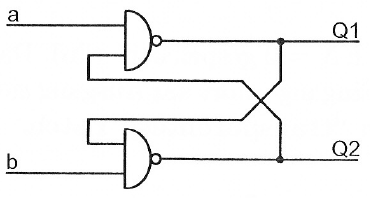
\includegraphics[width=0.5\textwidth]{../Anleitung/7-1.png}
    \caption{%
		\cite[Abbildung~7.1]{physik313-Anleitung}
    }
    \label{fig:7-1}
\end{figure}

\begin{table}
    \centering
    \begin{tabular}{cc|cc}
        $a$ & $b$ & $Q_1$ & $Q_2$ \\
        \hline
        0 & 0 & 1 & 1 \\
        0 & 1 & 1 & 0 \\
        1 & 0 & 0 & 1 \\
        1 & 1 & 1/0 & 0/1
    \end{tabular}
    \caption{%
        Funktionstafel für das in Abbildung~\ref{fig:7-1} gezeigte Flip-Flop 
    }
    \label{tab:Aufgabe_F}
\end{table}

Wie in Tabelle~\ref{tab:Aufgabe_F} zu sehen ist, gibt es für $a = b = 1$ zwei
mögliche Ausgangseinstellungen.

\FloatBarrier
\subsection{Aufgabe G}

\begin{problem}
    Zeichnen Sie ein 4-Bit-Schieberegister auf, das seriell geladen wird.
\end{problem}

Die Schaltung des seriell geladenen Schieberegisters ist in
Abbildung~\ref{fig:G-Schieberegister} zu sehen.

\begin{figure}
    \centering
    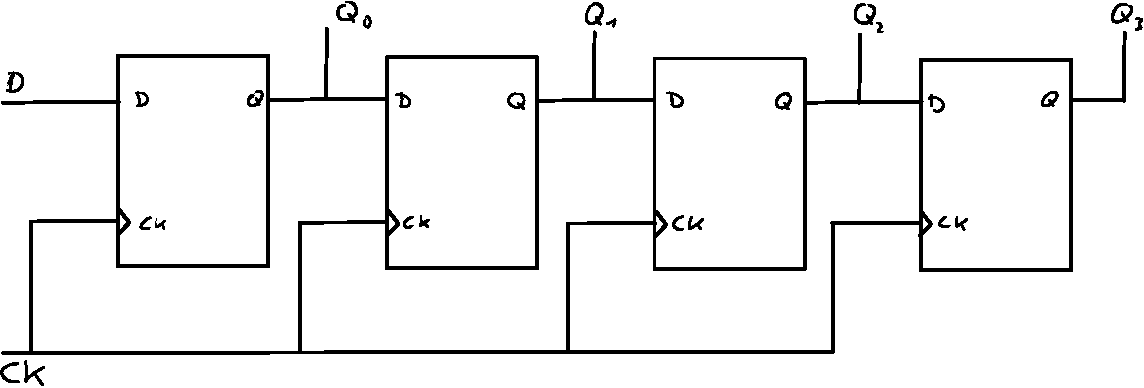
\includegraphics[width=\textwidth]{../Zeichnungen/G-Schieberegister.pdf}
    \caption{%
        Seriell geladenes Schieberegister
    }
    \label{fig:G-Schieberegister}
\end{figure}

\FloatBarrier
\subsection{Aufgabe H}

\begin{problem}
    Entwerfen Sie ein 4-Bit-Schieberegister, das parallel geladen werden kann
    (d.h. alle Bits gleichzeitig, wenn eine Steuerleitung „\textsc{load}“ auf 1
    ist). Benutzen Sie dazu die unten [Abbildung~\ref{fig:7-H}] abgebildeten
    kombinierten Schaltelemente, die auch auf dem Schaltbrett zur Verfügung
    stehen.
\end{problem}

Die Schaltung ist in Abbildung~\ref{fig:H-Schieberegister} zu sehen.

Steht \textsc{load} auf 1 wird beim entsprechenden Takt jedes Bit gleichzeitig
von $D_i$ aus geladen, da der Multiplexer diese Quelle auswählt. Steht
\textsc{load} auf 0, wirkt diese Schaltung wie das in
Abbildung~\ref{fig:G-Schieberegister} gezeigte seriell geladene Schieberegister.

\begin{figure}
    \centering
    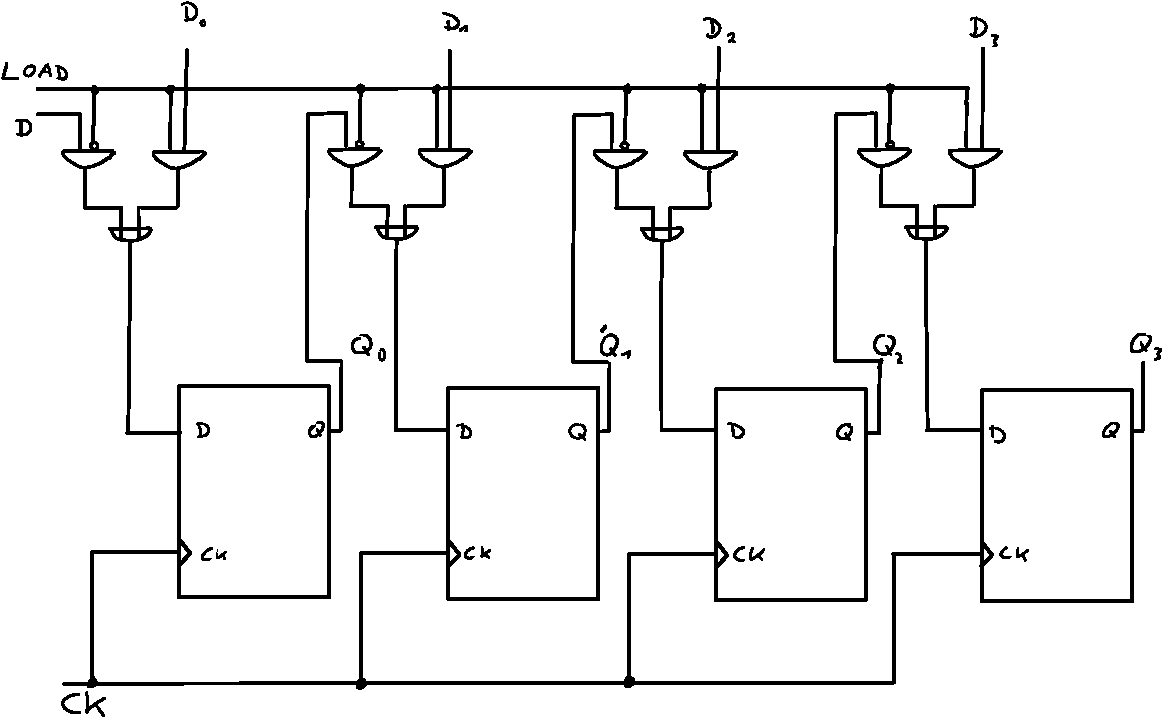
\includegraphics[width=\textwidth]{../Zeichnungen/H-Schieberegister.pdf}
    \caption{%
        Parallel und seriell ladbares Schieberegister
    }
    \label{fig:H-Schieberegister}
\end{figure}

\FloatBarrier
\subsection{Aufgabe K}

\begin{problem}
	Welche logische Funktion wir[d] durch diese Schaltung [in
	Abbildung~\ref{fig:7-7}] realisiert? Welche Aufgabe haben die Dioden?
	Überprüfen Sie, ob auch hier noch die Ausgangspegel korrekt sind.
\end{problem}

\begin{figure}[htbp]
	\centering
	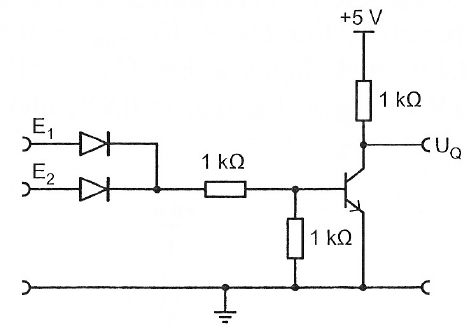
\includegraphics[width=.5\linewidth]{../Anleitung/7-7.png}
	\caption{%
		\cite[Abbildung~7.7]{physik313-Anleitung}
	}
	\label{fig:7-7}
\end{figure}

Die die logische Funktion des Schaltung ist eine \tnor-Funktion.

Die Dioden
haben die Funktion die einkommenden Spannungen nur an das Gatter
weiterzuleiten. Die Eingangsspannung soll von beiden Eingängen auf $\UEH$
gezogen werden können, jedoch sollen die Eingänge voneinander entkoppelt sein,
sie sollen ja Eingänge sein.

\paragraph{Spannungslevel}

Wenn nur $\UL$ auf beiden Eingängen ist, liegt eine maximale Spannung von
\SI{.2}{\volt} an, da die Siliziumdioden schon \SI{.6}{\volt} verschlingen.
Dies reicht nicht mehr aus, um den Transistor zu schalten, am Ausgang werden
fast die vollen \SI{5}{\volt} anliegen.

Wenn einer der der Eingänge auf $\UL$ geschaltet ist, dann mindestens
\SI{2.4}{\volt}. Nach der Diode sind immer noch \SI{1.8}{\volt} da. Dies sollte
reichen, um den Transistor zu schalten. $\UBE$ ist dann nur noch
\SI{.7}{\volt}, so dass folgender Strom fließt:
\[
	\IB = \frac{\SI{1.8}\volt - 2 \cdot \SI{.7}\volt}{\SI1{\kilo\ohm}}
	= \SI{.4}{\milli\ampere}
\]

Mit einer Stromverstärkung von $\beta = 100$ sind dies $\IB =
\SI{40}{\milli\ampere}$. Dabei würde an $\RC$ eine Spannung von \SI{40}{\volt}
abfallen. Da nur \SI{5}{\volt} anliegen, wird sicher ein \thigh{} am Ausgang
anliegen.

\FloatBarrier
\subsection{Aufgabe L}

\fehlt

\FloatBarrier
\subsection{Aufgabe M}

\begin{problem}
	Wie funktioniert der CMOS-Inverter (Abbildung~\ref{fig:7-9})? Benutzen Sie
	die angegebenen Kennlinien.
\end{problem}

\begin{figure}[htbp]
	\centering
	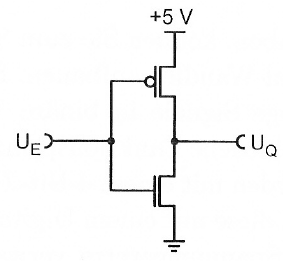
\includegraphics[width=.3\linewidth]{../Anleitung/7-9.png}
	\caption{%
		\cite[Abbildung~7.9]{physik313-Anleitung}
	}
	\label{fig:7-9}
\end{figure}

Wenn eine Eingangsspannung anliegt, also ein \thigh, sperrt der obere FET, der
untere FET wird durchgeschaltet. Somit fällt die Betriebsspannung am oberen FET
ab, Ausgang ist ein \tlow.

Wenn keine Eingangsspannung anliegt, also ein \tlow, wird der Obere
durchgeschaltet, der Untere gesperrt. Damit fällt die Betriebsspannung am
unteren ab, Ausgang ist ein \thigh.

Die Kennlinien sind so extrem, dass sich hier ein digitales Verhalten zeigt.

\FloatBarrier
\subsection{Aufgabe N}

\begin{problem}
	Welche logische Funktion ist mit dem Gatter in Abbildung~\ref{fig:7-10}
	realisiert?
\end{problem}

\begin{figure}[htbp]
	\centering
	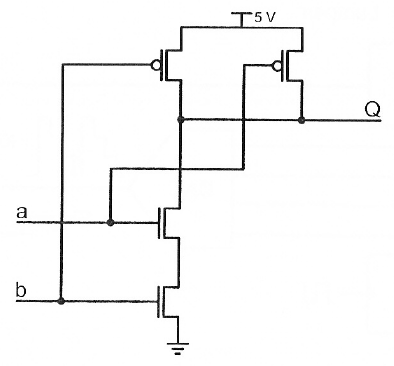
\includegraphics[width=.5\linewidth]{../Anleitung/7-10.png}
	\caption{%
		\cite[Abbildung~7.10]{physik313-Anleitung}
	}
	\label{fig:7-10}
\end{figure}

Legen wir doch eine Tabelle an. Dazu gehen wir Schritt für Schritt durch:

\paragraph{A und B \tlow}

n-MOS links und rechts sind durchgeschaltet. Daher fällt über ihnen keine
Spannung ab. Die p-MOS oben und unten sind gesperrt, daher fällt über ihnen
Spannung ab. Ausgang ist \thigh.

\paragraph{A und B \thigh}

Genau invers, also fällt die Spannung über den ersten MOSFETs ab, womit der
Ausgang \tlow ist.

\paragraph{A \thigh{} und B \tlow}

n-MOS links ist offen, n-MOS rechts ist gesperrt. p-MOS oben ist offen, p-MOS
unten ist gesperrt.

Somit fällt viel Spannung unten ab, oben ist ein Weg offen. Ausgang ist \thigh.

\paragraph{A \tlow{} und B \thigh}

n-MOS links ist gesperrt, rechts ist offen. p-MOS oben ist gesperrt, unten ist
offen.

Somit wie oben, \thigh

\paragraph{Zusammenfassung}

Wir erhalten:

\begin{tabular}{c|cc}
	A \textbackslash{} B & 0 & 1 \\
	\hline
	0 & 1 & 1 \\
	1 & 1 & 0
\end{tabular}

Somit handelt es sich um ein \tnand-Gatter.

\FloatBarrier
\subsection{Aufgabe O}

\begin{problem}
	Wie lauten die Bool'schen Ausdrücke für Summe und Übertrag eines
	Halbaddierers?
\end{problem}

Einen Übertrag gibt es nur, wenn beide Summanden \thigh{} sind. Somit ist der
Übertrag:
\[
	U := a \mand b
\]

Die Summe ist ein \txor. Also:
\[
	S := a \mxor b
\]

\FloatBarrier
\subsection{Aufgabe P}

\begin{problem}
	Schreiben Sie die Funktionstafel auf für einen Volladdierer, der auch den
	Übertrag des vorhergehenden Bits mit verarbeitet.
\end{problem}

Der Volladdierer bekommt nicht nur die beiden Stellen $a$ und $b$ geliefert,
sondern auch $\Uin$, den Übertrag der vorherigen Rechnung. Der Volladdierer
addiert diese drei Zahlen auf. Da sie im Bereich 0 bis 3 liegen, braucht er
zwei Stellen als Ausgabe. Das ist einmal Summe und $\Uout$, der Übertrag des
Ergebnisses.

\begin{tabular}{ccc|cc}
	$a$ & $b$ & $\Uin$ & $\Uout$ & $S$ \\
	\hline
	0 & 0 & 0 & 0 & 0 \\
	0 & 0 & 1 & 0 & 1 \\
	0 & 1 & 0 & 0 & 1 \\
	0 & 1 & 1 & 1 & 0 \\
	1 & 0 & 0 & 0 & 1 \\
	1 & 0 & 1 & 1 & 0 \\
	1 & 1 & 0 & 1 & 0 \\
	1 & 1 & 1 & 1 & 1 \\
\end{tabular}

\begin{small}
	Für die Bearbeitung dieser Aufgabe habe ich mir
	\cite{wikipedia/Volladdierer} angeschaut. Die Tabelle habe ich jedoch nicht
	kopiert, sondern aus der Erklärung im ersten Absatz des Artikels selbst
	erstellt.
\end{small}

\FloatBarrier
\subsection{Aufgabe Q}

\begin{problem}
	Geben Sie ein Blockschaltbild an für einen Volladdierer, der aus zwei
	Halbaddierern zusammengesetzt ist.
\end{problem}

Der Volladdierer soll, wie in der vorherigen Aufgabe beschrieben, drei Zahlen
addieren. Dazu werden erst einmal $a$ und $b$ addiert, zur Zwischensumme $Z$
und ihrem Übertrag $U_Z$. Anschließend werden werden der vorherige Übertrag
$\Uin$ mit der Zwischensumme addiert. Als Ergebnis kommen die Summe $S$ und ein
weiterer Übertrag $U_S$ heraus. Die beiden Überträge können jedoch nicht beide
\thigh{} sein. Somit reicht es, sie mit einem \tor-Gatter zu verknüpfen.

Dies ist in Abbildung~\ref{fig:Q-Volladdierer} gezeigt.

\begin{figure}[htbp]
	\centering
	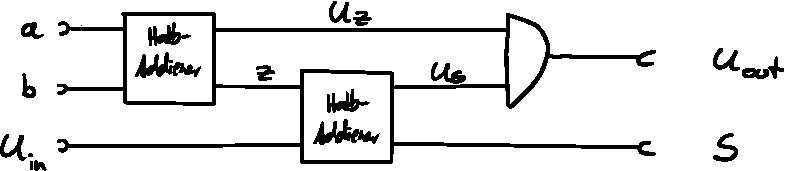
\includegraphics{../Zeichnungen/Q-Volladdierer.pdf}
	\caption{%
		Blockschaltbild für den Volladdierer. Mit Denkanstoß von
		\cite{wikipedia/Volladdierer}.
	}
	\label{fig:Q-Volladdierer}
\end{figure}

\FloatBarrier
\subsection{Aufgabe R}

\begin{problem}
	Entwerfen Sie ein Schaltschema eines seriellen Addierwekes wie oben
	beschrieben. Mit den auf dem Schaltbrett vorhandenen Elementen ist es nicht
	möglich, zwei Register aufzubauen, die man beide parallel laden kann.
	Füllen Sie deswegen das eine Summandenregister, welches gleichzeitig als
	Ergebnisregister dient, indem Sie zunächst den ersten Summanden zu Null
	hinzuaddieren.
\end{problem}

\begin{figure}[htbp]
	\centering
	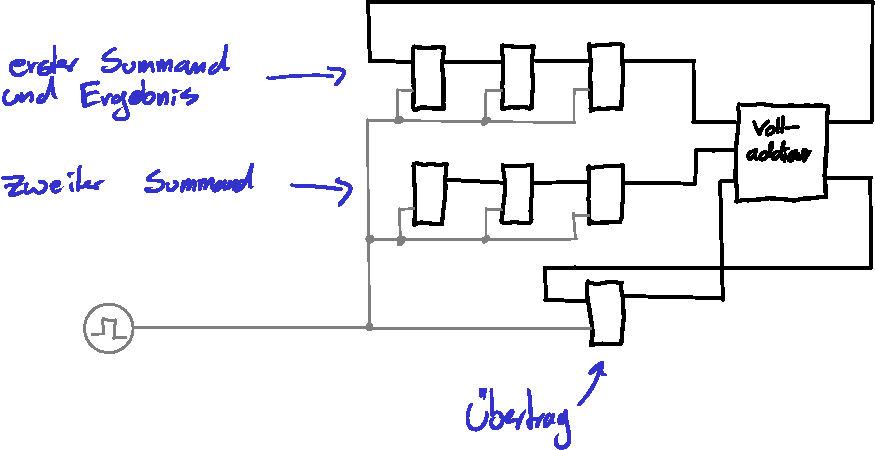
\includegraphics{../Zeichnungen/R-Addierer.pdf}
	\caption{%
		Blockschaltbild für die vollständige Addiererschaltung.
	}
	\label{fig:R-Addierer}
\end{figure}

%%%%%%%%%%%%%%%%%%%%%%%%%%%%%%%%%%%%%%%%%%%%%%%%%%%%%%%%%%%%%%%%%%%%%%%%%%%%%%%
%                                Durchführung                                %
%%%%%%%%%%%%%%%%%%%%%%%%%%%%%%%%%%%%%%%%%%%%%%%%%%%%%%%%%%%%%%%%%%%%%%%%%%%%%%%

\section{Durchführung}

\subsection{Aufgabe d}

Wir sollen in diesem Versuch einen Halbaddierer aus \tnand-Gattern
zusammensetzen. Für diesen brauchen wir \tand- und \tor-Gatter. Diese sind in
Abbildung~\ref{fig:and} und \ref{fig:or} gezeigt.

\begin{figure}[htbp]
	\centering
	\begin{minipage}{.45\linewidth}
		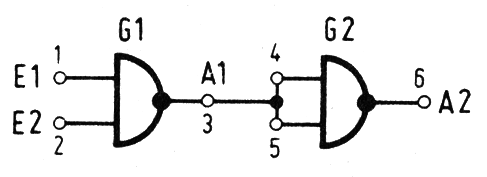
\includegraphics[width=\linewidth]{../Gatter/AND.png}
		\caption{%
			\tand-Gatter.
			\cite[Seite~20]{wirsum/experimente_schaltglieder}
		}
		\label{fig:and}
	\end{minipage}
	\hfill
	\begin{minipage}{.45\linewidth}
		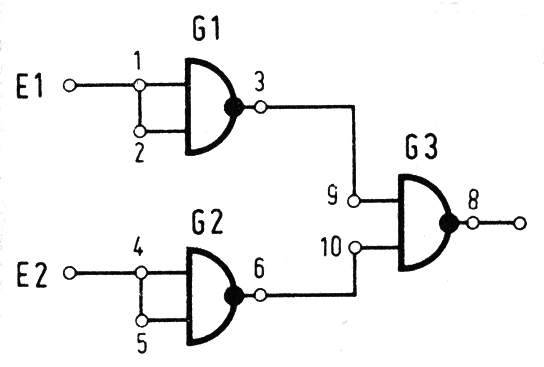
\includegraphics[width=\linewidth]{../Gatter/OR.png}
		\caption{%
			\tor-Gatter
			\cite[Seite~21]{wirsum/experimente_schaltglieder}
		}
		\label{fig:or}
	\end{minipage}
\end{figure}

%%%%%%%%%%%%%%%%%%%%%%%%%%%%%%%%%%%%%%%%%%%%%%%%%%%%%%%%%%%%%%%%%%%%%%%%%%%%%%%
%                                  Literatur                                  %
%%%%%%%%%%%%%%%%%%%%%%%%%%%%%%%%%%%%%%%%%%%%%%%%%%%%%%%%%%%%%%%%%%%%%%%%%%%%%%%

\FloatBarrier
\IfFileExists{\bibliographyfile}{
	\bibliography{\bibliographyfile}
}{}

\end{document}

% vim: spell spelllang=de tw=79
